\chapter{Introdução}
A maneira que observamos a natureza e o universo sempre dependeu de instrumentos. Microscópios trouxeram a noção de que micro-organismos extremamente pequenos existiam, nos permitiram descobrir as bactérias, as formas de vida mais comuns do planeta. Telescópios nos deram habilidades de observar o sistema solar descobrir as órbitas dos planetas e formular a noção de gravidade de Newton. %\cite{newton1687philosophiae}. 

Mas nem sempre essas descobertas acontecem de propósito. Em 1930, o físico Karl Jansky descobriu sinais de rádio que causava a inferência das chamadas telefônicas com estática, e esse sinal era originado no centro da nossa Via Láctea, com a maior parte dos sinais de rádio vindos da constelação de sagitário. Uma descoberta por acaso, feita sem querer por alguém que estava preparado para entender o que havia encontrado, uma serendipidade.

Assim como o sol emite radiação eletromagnética na forma de ondas de luz. Também emite frequências maior e menor, como rádio, raios-X, raios gama, entre outras. E graças a Jansky, que inaugurou a radioastronomia, fomos capazes de observar o universo com os radiotelescópios, que nos permite ver, de explosões aos bips de pulsares \cite{jansky1932directional}. Assim, podemos ver em outros comprimentos de ondas além da luz visível e com isso observar novos fenômenos, como por exemplo, observações de raio-x que mostram buracos negros rasgando as estrelas \cite{200814} e quasares \cite{mortlock2011luminous}, o quanto a radiação infravermelha atravessa a Via Láctea e nos mostra o que tem por trás dela \cite{wright2010wide}. 

O que a descoberta da radioastronomia teve de serendipidade, a descoberta das ondas gravitacionais (Gravitational waves) (GW) teve de proposital. Começando por Einstein, em 1915, quando ele adicionou a gravidade à teoria da relatividade. Publicando a Teoria da Relatividade Geral, Einstein concluiu que a gravidade não era uma força, mas sim a deformação do espaço tempo, e essa deformação do espaço deveria viajar pelo universo como uma onda, viajando na velocidade da luz \cite{albert1920realtivity}.

De forma geral, as ondas gravitacionais podem ser pensadas como as ondas criadas quando jogamos pedras na superfície de um lago. Essas ondas são perturbações na geometria do próprio espaço-tempo emitidas por colisões violentas que acontecem no universo, que se propagam à velocidade da luz, carregando informações sobre suas origens, bem como pistas sobre a natureza da própria gravidade \cite{LSC-VIRGO, abbott2016observation}.

A real existência dessas ondas ficou por um longo período restrito a discussões teóricas. Até por volta de 1960, descobertas astronômicas (quasares, pulsares, radiação cósmica de fundo) e novos experimentos impulsionaram a relatividade geral, para a linha de frente. Neste período foi descoberto a diminuição no período orbital do pulsar binário Hulse-Taylor em uma taxa consistente com a predição da relatividade geral da perda de energia por ondas gravitacionais \cite{weisberg2004relativistic}, e essa havia sido a primeira detecção indireta de ondas gravitacionais da historia da ciência.

Na prática, é extremamente difícil detectar diretamente a presença de ondas gravitacionais porque o alongamento e a compressão do espaço-tempo é muito pequeno. Em uma onda gravitacional típica, supõe-se que esta amplitude de deformação deva ser, aproximadamente, dez mil vezes menor que o diâmetro de um próton \cite{LSC-VIRGO}.

Para observar esse tipo de fenômeno precisamos do Observatório de Ondas Gravitacionais por Interferometria a Laser (Advanced Laser Interferometer Gravitational Wave Observatory) (aLIGO) \cite{PhysRevLett.116.131103,0264-9381-32-7-074001}, que recentemente, até o momento, tem anunciado a detecção de ondas gravitacionais a partir de medidas de uma série de eventos cósmicos que envolvem colapso de sistemas binários formados por objetos compactos tais como buracos negros \cite{abbott2016observation,ligo2016gw151226,scientific2017gw170104,abbott2017gw170814}, e estrelas de nêutrons \cite{abbott2017gw170817}, que são consistentes com as previsões da relatividade geral de Einstein.

O observatório LIGO tem dois centros, com formato em L. Um posicionado em Washington e outro em Louisiana nos Estados Unidos, na quina desse L um espelho divide um feixe de laser em duas partes, que percorrem, cada uma, um dos tubos de 4 quilômetros e encontra um espelho lá no final. Quando as ondas de laser voltam, elas se anulam e desaparecem, caso um dos tubos seja deslocado por causa de uma deformação do espaço e do tempo, ele muda a distância percorrida pelo laser, e o sinal deixa de ser cancelado, como ilustra a Figura~\ref{figinterferometer}. Para garantir que a deformação foi causada por uma onda gravitacional e não um terremoto ou outro problema, o mesmo sinal tem que ser observado nos dois centros \cite{PhysRevLett.116.131103}. 

\begin{figure}[ht]
\centering
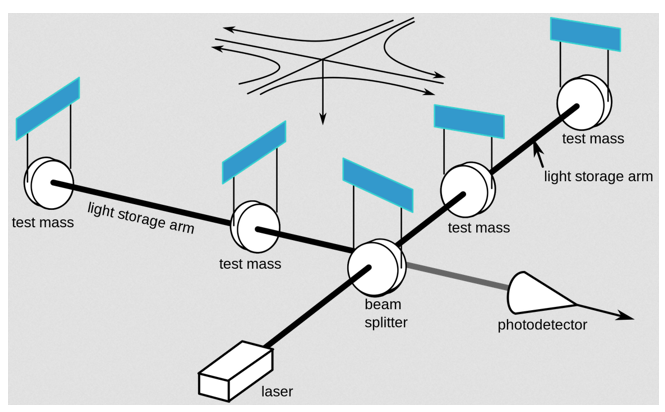
\includegraphics[width=1\textwidth]{figuras/interferometro.png}
\caption{Diagrama de um projeto básico de interferômetro. [Image: LIGO]}
\label{figinterferometer}
\end{figure}
 
Após a parada do LIGO nos períodos de 2010 à 2015 o observatório foi parado para passar por um upgrade na capacidade de detecção e logo no inicio de suas atividade ele captou o primeiro sinal de uma colisão de buracos negros, há 1,3 bilhão de anos luz daqui, que levando ao prêmio Nobel de Física em 2017 \cite{abbott2016observation}. 
 
Quando um objeto denso e massivo é acelerado, ele cria ondas gravitacionais como as ondas que uma pedra lançada em um lago produz, e de acordo com Einstein, nada é mais denso e massivo do que um buraco negro e em um sistema binário, dois buracos negros giram um ao redor do outro. Na primeira detecção que foi observada \cite{abbott2016observation}, um deles tinha a massa de 36 sóis e o outro de 29 conforme eles giravam em órbita, emitiam ondas gravitacionais e com isso perderam energia, conforme perderam energia, se aproximaram ainda mais e giraram ainda mais rápido, quanto mais se aproximavam, mais energia perdiam e mais ondas emitiam e mais se aproximavam cada vez mais rápido até colidirem.

No final da explosão o buraco resultante ficou com 62 massas solares, os 3 sóis de diferença foram convertidos em ondas gravitacionais. Conforme os buracos negros se aceleram antes da colisão, as ondas que emitem ficam cada vez mais intensas e cada vez mais frequentes, até virarem um gorjeio, que marca a colisão, um gorjeio emitido há mais de 1 bilhão de anos, uma explosão tão forte, que chacoalhou o espaço e o tempo e conseguimos captar daqui.

A descoberta das ondas gravitacionais são mais uma confirmação da Teoria da Relatividade Geral que se soma às outras confirmações das Teoria de Einstein, tais como a deflexão da luz ao passar com objetos massivos como estrelas, lentes gravitacionais, a explicação do desvio do periélio do planeta Mercúrio, efeitos relativísticos nas órbitas dos planetas, buracos negros, etc. 

Os efeitos Relativísticos de natureza gravitacionais são de grande importância à atual tecnologia e com aplicação à vida diária das pessoas. Um dos principais resultados da Teoria da Relatividade Geral foi a possibilidade de permitir a localização de coordenadas na superfície de planetas com extrema precisão (o equivalente ao georreferenciamento, contudo extraterrestre, a partir da Terra). A localização de coordenadas na superfície de planetas é uma das aplicações tecnológicas que só foi possível com uso da Teoria da Relatividade Geral. O resultado de tal tecnologia aplicado ao caso do planeta Terra foi o desenvolvimento da tecnologia do Sistema de Posicionamento Global GPS (Global Positioning System).

Agora temos a confirmação de que as ondas gravitacionais, as quais tem sido um objetivo de estudo perseguido por cerca de 100 anos, realmente existem, e sabemos como detectá-las. Em pouco tempo teremos detectores como LIGO em órbita da terra, com sensores há milhares de quilômetros de distância, capazes de detectar ondas gravitacionais ainda menores. Agora podemos captar as ondas emitidas pela explosão de supernovas ou pela fusão de estrelas de nêutrons formando buracos negros.

\section{Delimitação do Tema}

A natureza nem sempre pode ser observada em sua plenitude, mas sempre poderá ser simulada computacionalmente desde que existam os apropriados modelos computacionais. Neste sentido, a computação científica e numérica desempenha o papel de ferramenta fundamental da área da ciência da computação para o entendimento da natureza, explicitando fenômenos e dinâmicas muitas vezes não possíveis de serem observados pela limitada capacidade humana de observação.

Capacidade essa que também não pode acompanhar a avalanche de informações produzidas por muitos dos experimentos de física e astronomia de hoje. Os quais, alguns deles registram terabytes de dados todos os dias e a quantidade de dados produzida a cada dia está apenas aumentando. O Square Kilometer Array, um radiotelescópio programado para ser ativado em meados deste ano, será capaz de gerar um tráfego de dados maior que a Internet inteira a cada ano \cite{ska,ska-dewdney2009square}.

Atualmente muitos cientistas recorrem à inteligência artificial para obter ajuda. Sistemas de Inteligência Artificial (AI) como redes neurais artificiais (RNA), que são redes de neurônios simuladas por computador que imitam a função do cérebro, as quais, podem atravessar montanhas de dados, destacando anomalias e detectando padrões que humanos nunca poderiam ter visto.

Por esse motivo, os pesquisadores passaram a depender de tecnologias integradas para serem capazes de lidar com esse grande fluxo de dados e o uso efetivo desses dados tornou possível aprimorar os métodos de pesquisa, transformando a forma de se fazer ciência. E a IA se insere nesse contexto justamente para auxiliar os pesquisadores nessa missão. Ela nos permite extrair novos insights das informações disponíveis para melhorar a busca de anomalias e detectar padrões que humanos nunca poderiam ter visto.

Nos últimos anos, as técnicas de IA, em particular as redes neurais, foram investigadas como um método para substituir ou complementar as técnicas tradicionais de filtragem por coincidência \cite{1057571}, usadas para detectar sinais de ondas gravitacionais de fusão de buracos negros \cite{shen2017denoising,PhysRevLett.120.141103,krastev2019real,gebhard2019convolutional,mukund2017transient,kim2015application,george2018deep}. Por meio da RNA, os pesquisadores conseguiram otimizar processos que antes levariam semanas e, agora, podem ser realizados em questão de segundos. Essa tecnologia se baseia na capacidade de um software substituir a força humana na realização de tarefas complexas.


\section{Problema de Pesquisa}

A busca da detecção de ondas gravitacionais continua intensa, a análise e o tratamento computacional destas informações encontram-se na crisa da onda da tecnologia computacional para o entendimento de tal processo.

Para que seja possível a detecção de ondas gravitacionais é necessário um grande esforço contínuo dos detectores e das instalações astronômicas, a natureza sensível a tempo dessas análises requer algoritmos que possam detectar e caracterizar esses eventos em tempo real. O custo computacional das buscas usando o método de filtragem por coincidência, aumenta significativamente quando é necessário a busca por sinais em uma grande quantidade de dados.

Por outro lado, por mais que os métodos que utilizam as redes neurais profundas possam ser mais rápidos que a filtragem por coincidência, ainda necessitam do uso da computação de alto desempenho (HPC do inglês, high performance computing). A Própria natureza das redes profundas a tornam um processo custoso quanto ao seu preparo e desenvolvimento, as tornando obsoletas em comparação a outros tipos de redes neurais.

Os métodos desenvolvidos com redes neurais podem ser otimizados e acelerados ainda mais, no entanto, esta pode não ser uma tarefa trivial. Nos dias de hoje é possível executar softwares de inteligencia artificial em hardwares comerciais mais simples e que estão disponíveis no marcado, portando não seria difícil executar uma busca por ondas gravitacionais em casa com o uso de um laptop, graças a redes neurais mais simples e otimizadas.

\section{Objetivos}
A seguir serão apresentados os objetivos geral (OG) e específicos (OE) que nortearão a condução desta pesquisa.

\subsection{Objetivo Geral}

A presente pesquisa tem como objetivo geral o desenvolvimento de procedimentos computacionais baseados em Machine Learning para a detecção de ondas gravitacionais, contribuindo para uma nova área de pesquisa computacional designada de Astroinformatica com o desenvolvimento de um classificados binário capaz de classifica as reais medidas das ondas gravitacionais.

\subsection{Objetivos Específicos}
Para atingir o objetivo geral foram definidos os seguintes objetivos específicos: 
\begin{itemize}

\item Investigação e obtenção dos modelos das ondas gravitacionais descobertas pelo LIGO;
\item Simulações computacionais de ondas gravitacionais em uma plataforma baseada em hardware comercial;
\item Tratamento dos dados simulados e obtidos do LIGO para o treinamento e validação da RNA;
\item E Desenvolvimento e implementação do Comitê de Redes Neurais Artificiais para a classificação de sinais de ondas gravitacionais nos dados reais do LIGO em uma plataforma CPU comercial;

\end{itemize}
\section{Justificativa}

Com base em todas as considerações descritas, precisamos de um novo paradigma para superar as limitações e os desafios computacionais dos algoritmos de detecção de GW existentes, eliminando assim a necessidade do uso de super computadores, e libertando a pesquisa de ondas gravitacionais a qualquer ambiente computacional.

Um candidato ideal para este feito seria a Machine Learning, mais especificamente um Comitê de Redes Neurais Artificiais, a qual hoje é tendencia no mercado, que é uma área  altamente escalável que pode aprender diretamente a partir de dados brutos, sem qualquer recurso manual de engenharia, usando camadas hierárquicas de redes, em combinação com técnicas de otimização baseadas em retro-propagação e gradiente descendente~\cite{barca2005treinamento}. 

A Machine Learning, especialmente com o auxílio da computação GPU, que é encontrada na maioria dos hardwares pessoais, alcançou recentemente um imenso sucesso em aplicações comerciais e em Inteligência Artificial \cite{esteva2017dermatologist, moravvcik2017deepstack, van2016wavenet, 10.1007/978-3-319-44188-7_16}, e também tem sido aplicado em astrofísica \cite{shen2017denoising,PhysRevLett.120.141103,krastev2019real,gebhard2019convolutional,mukund2017transient,kim2015application,george2018deep,george2017glitch, george2017deepA}.

\section{Organização do trabalho}

O presente trabalho está organizado em 5 capítulos e um apêndice, a saber: Fundamentação Teórica, Metodologia, Resultados, Conclusão e Apêndice A. A seguir, são descritos resumidamente o conteúdo de cada um.

Na Fundamentação Teórica são apresentados conceitos sobre ondas gravitacionais e redes neurais artificiais. Na seção sobre ondas gravitacionais, é descrito uma breve explicação do que são ondas gravitacionais, suas fontes, tipos de sinais e como gerar formas de ondas com cálculos físicos. Na seção das redes neurais, descreve-se o neurônio artificial, algumas arquiteturas de redes e o processo de aprendizagem utilizado no trabalho (retro-propagação). 

No capítulo Metodologia, são descritas as ferramentas computacionais utilizadas, o tratamento dos dados obtidos do LIGO e o processo de geração de formas de ondas, o processo ajustes de parâmetros e de aprendizagem das redes neurais geradas (MLPs) e o arranjo das MLPs com o comitê de redes neurais.

O capítulo Resultados apresenta os resultados obtidos com a aplicação dos dados reais do LIGO sobre o comitê de redes neurais treinadas, mostra também as arquiteturas de redes neurais desenvolvidas e a que melhor se adequou ao estudo, qual o melhor processo para a realização do treinamento das redes neurais e os critérios que levaram a esta descoberta.

No capítulo Conclusão são apresentados discussões sobre o trabalho como todo, ressaltando alguns detalhes observados nos Resultados, apresenta quais os ganhos e possíveis trabalhos futuros com descobertas já preestabelecidas.

No Apêndice A é mostrado os gráficos de score gerados pelo comitê de redes neurais para cada uma das ondas gravitacionais obtidas do LIGO utilizadas neste trabalho.